\definecolor{Gray}{rgb}{ .949,  .949,  .949}
\newcolumntype{g} {>{\columncolor{Gray}}c}
\chapter{Análisis de Semejantes}

Tal y como se ha reflejado en la introducción, el proceso a seguir para obtener un diseño preliminar será el análisis de semejantes.
Este análisis consiste en crear una base de datos de aeronaves ya existentes, cuyas características sean similares a las que podría tener la nuestra, de manera que mediante un análisis estadístico se pueda obtener una primera aproximación de algunas características de nuestra aeronave.

\section{Estudio de Aeronaves de Referencia}

Dado que el objetivo es el diseño de un helicóptero no tripulado de 450 kg de \emph{MTOW}, los vehículos a analizar serán helicópteros de una masa similar, en torno a 400-500 kg, pero al no existir una cantidad suficiente dentro de este margen, se ha decidido ampliar este.
En las tablas \ref{ASomega} y \ref{AS} se encuentran los helicópteros seleccionados para el análisis.

%PROBLEMAS CON LAS TABLAS, BUSCAR COMO ARREGLAR EL DESASTRE DE TABLA QUE NO ENTRA, TAL VEZ DIVIDIRLO EN 2 SEA SUFICIENTE
\begin{table}[htbp]
	\centering
	\begin{tabular}{|l|c|c|c|c|c|c|c|}
		\hline
		\rowcolor[rgb]{ .851,  .851,  .851} MODELO & \multicolumn{1}{l|}{MTOW[kg]} & \multicolumn{1}{l|}{d[m]} & \multicolumn{1}{l|}{$\Omega$ [rad/s]} & \multicolumn{1}{l|}{b} & \multicolumn{1}{l|}{$b_a$} & \multicolumn{1}{l|}{$h_{max}$[m]} & \multicolumn{1}{l|}{$V_{max}$[km/h]} \\ \hline
		\rowcolor[rgb]{ .949,  .949,  .949} SA-200 Weasel & \cellcolor[rgb]{ 1,  1,  1}70 & \cellcolor[rgb]{ 1,  1,  1}2,07 & \cellcolor[rgb]{ 1,  1,  1}167,55 & \cellcolor[rgb]{ 1,  1,  1}2 & \cellcolor[rgb]{ 1,  1,  1}6 & \cellcolor[rgb]{ 1,  1,  1}3100 & \cellcolor[rgb]{ 1,  1,  1}167 \\
		\hline
		\rowcolor[rgb]{ .949,  .949,  .949} Yamaha R-50 & \cellcolor[rgb]{ 1,  1,  1}90 & \cellcolor[rgb]{ 1,  1,  1}3,07 & \cellcolor[rgb]{ 1,  1,  1}88,6 & \cellcolor[rgb]{ 1,  1,  1}2 & \cellcolor[rgb]{ 1,  1,  1}2 & \cellcolor[rgb]{ 1,  1,  1}300 & \cellcolor[rgb]{ 1,  1,  1}VACÍO \\
		\hline
		\rowcolor[rgb]{ .949,  .949,  .949} R-350 & \cellcolor[rgb]{ 1,  1,  1}150 & \cellcolor[rgb]{ 1,  1,  1}3,5 & \cellcolor[rgb]{ 1,  1,  1}82,86 & \cellcolor[rgb]{ 1,  1,  1}3 & \cellcolor[rgb]{ 1,  1,  1}2 & \cellcolor[rgb]{ 1,  1,  1}2500 & \cellcolor[rgb]{ 1,  1,  1}120 \\
		\hline
		\rowcolor[rgb]{ .949,  .949,  .949} SD 150 Hero & \cellcolor[rgb]{ 1,  1,  1}150 & \cellcolor[rgb]{ 1,  1,  1}3,5 & \cellcolor[rgb]{ 1,  1,  1}105,14 & \cellcolor[rgb]{ 1,  1,  1}3 & \cellcolor[rgb]{ 1,  1,  1}2 & \cellcolor[rgb]{ 1,  1,  1}4000 & \cellcolor[rgb]{ 1,  1,  1}90 \\
		\hline
		\rowcolor[rgb]{ .949,  .949,  .949} APID 55 & \cellcolor[rgb]{ 1,  1,  1}160 & \cellcolor[rgb]{ 1,  1,  1}3,3 & \cellcolor[rgb]{ 1,  1,  1}54,54 & \cellcolor[rgb]{ 1,  1,  1}2 & \cellcolor[rgb]{ 1,  1,  1}2 & \cellcolor[rgb]{ 1,  1,  1}3000 & \cellcolor[rgb]{ 1,  1,  1}90 \\
		\hline
		\rowcolor[rgb]{ .949,  .949,  .949} APID 60 & \cellcolor[rgb]{ 1,  1,  1}180 & \cellcolor[rgb]{ 1,  1,  1}3,3 & \cellcolor[rgb]{ 1,  1,  1}90,97 & \cellcolor[rgb]{ 1,  1,  1}2 & \cellcolor[rgb]{ 1,  1,  1}2 & \cellcolor[rgb]{ 1,  1,  1}3000 & \cellcolor[rgb]{ 1,  1,  1}110 \\
		\hline
		\rowcolor[rgb]{ .949,  .949,  .949} Camcopter S100 & \cellcolor[rgb]{ 1,  1,  1}200 & \cellcolor[rgb]{ 1,  1,  1}3,4 & \cellcolor[rgb]{ 1,  1,  1}130,73 & \cellcolor[rgb]{ 1,  1,  1}2 & \cellcolor[rgb]{ 1,  1,  1}2 & \cellcolor[rgb]{ 1,  1,  1}5500 & \cellcolor[rgb]{ 1,  1,  1}222 \\
		\hline
		\rowcolor[rgb]{ .949,  .949,  .949} Pelícano & \cellcolor[rgb]{ 1,  1,  1}200 & \cellcolor[rgb]{ 1,  1,  1}3,3 & \cellcolor[rgb]{ 1,  1,  1}81,22 & \cellcolor[rgb]{ 1,  1,  1}2 & \cellcolor[rgb]{ 1,  1,  1}2 & \cellcolor[rgb]{ 1,  1,  1}3600 & \cellcolor[rgb]{ 1,  1,  1}180 \\
		\hline
		\rowcolor[rgb]{ .949,  .949,  .949} DP 5X Wasp & \cellcolor[rgb]{ 1,  1,  1}227 & \cellcolor[rgb]{ 1,  1,  1}3,2 & \cellcolor[rgb]{ 1,  1,  1}127,33 & \cellcolor[rgb]{ 1,  1,  1}4 & \cellcolor[rgb]{ 1,  1,  1}4 & \cellcolor[rgb]{ 1,  1,  1}4100 & \cellcolor[rgb]{ 1,  1,  1}160 \\
		\hline
	\end{tabular}%
	\caption{Valores de diferentes parámetros de las aeronaves empleadas para el análisis de semejantes cuyos valores de velocidad de giro del rotor principal han sido publicados.}
	\label{ASomega}
\end{table}%

\begin{table}[htbp]
	\centering
	\begin{tabular}{|l|c|c|c|c|c|c|}
		\hline
		\rowcolor[rgb]{ .851,  .851,  .851} MODELO & \multicolumn{1}{l|}{MTOW[kg]} & \multicolumn{1}{l|}{d[m]} & \multicolumn{1}{l|}{b} & \multicolumn{1}{l|}{$b_a$} & \multicolumn{1}{l|}{$h_{max}$[m]} & \multicolumn{1}{l|}{$V_{max}$[km/h]} \\
		\hline
		\rowcolor[rgb]{ .949,  .949,  .949} Scout B1-100 & \cellcolor[rgb]{ 1,  1,  1}77 & \cellcolor[rgb]{ 1,  1,  1}3,2 & \cellcolor[rgb]{ 1,  1,  1}2 & \cellcolor[rgb]{ 1,  1,  1}2 & \cellcolor[rgb]{ 1,  1,  1}VACÍO & \cellcolor[rgb]{ 1,  1,  1}VACÍO \\
		\hline
		\rowcolor[rgb]{ .949,  .949,  .949} Neo S300 & \cellcolor[rgb]{ 1,  1,  1}85 & \cellcolor[rgb]{ 1,  1,  1}3 & \cellcolor[rgb]{ 1,  1,  1}3 & \cellcolor[rgb]{ 1,  1,  1}2 & \cellcolor[rgb]{ 1,  1,  1}VACÍO & \cellcolor[rgb]{ 1,  1,  1}VACÍO \\
		\hline
		\rowcolor[rgb]{ .949,  .949,  .949} Skeldar V-200 & \cellcolor[rgb]{ 1,  1,  1}235 & \cellcolor[rgb]{ 1,  1,  1}4,6 & \cellcolor[rgb]{ 1,  1,  1}2 & \cellcolor[rgb]{ 1,  1,  1}2 & \cellcolor[rgb]{ 1,  1,  1}3500 & \cellcolor[rgb]{ 1,  1,  1}140 \\
		\hline
		\rowcolor[rgb]{ .949,  .949,  .949} Tanan EADS & \cellcolor[rgb]{ 1,  1,  1}300 & \cellcolor[rgb]{ 1,  1,  1}5 & \cellcolor[rgb]{ 1,  1,  1}2 & \cellcolor[rgb]{ 1,  1,  1}2 & \cellcolor[rgb]{ 1,  1,  1}4000 & \cellcolor[rgb]{ 1,  1,  1}150 \\
		\hline
		\rowcolor[rgb]{ .949,  .949,  .949} SVU-200 & \cellcolor[rgb]{ 1,  1,  1}360 & \cellcolor[rgb]{ 1,  1,  1}4,92 & \cellcolor[rgb]{ 1,  1,  1}4 & \cellcolor[rgb]{ 1,  1,  1}2 & \cellcolor[rgb]{ 1,  1,  1}4200 & \cellcolor[rgb]{ 1,  1,  1}209 \\
		\hline
		\rowcolor[rgb]{ .949,  .949,  .949} Cicare 7B & \cellcolor[rgb]{ 1,  1,  1}430 & \cellcolor[rgb]{ 1,  1,  1}6,28 & \cellcolor[rgb]{ 1,  1,  1}2 & \cellcolor[rgb]{ 1,  1,  1}2 & \cellcolor[rgb]{ 1,  1,  1}3000 & \cellcolor[rgb]{ 1,  1,  1}194 \\
		\hline
		\rowcolor[rgb]{ .949,  .949,  .949} Robinson R-22 & \cellcolor[rgb]{ 1,  1,  1}622 & \cellcolor[rgb]{ 1,  1,  1}7,67 & \cellcolor[rgb]{ 1,  1,  1}2 & \cellcolor[rgb]{ 1,  1,  1}2 & \cellcolor[rgb]{ 1,  1,  1}4267 & \cellcolor[rgb]{ 1,  1,  1}188 \\
		\hline
		\rowcolor[rgb]{ .949,  .949,  .949} VSR700 & \cellcolor[rgb]{ 1,  1,  1}680 & \cellcolor[rgb]{ 1,  1,  1}7,2 & \cellcolor[rgb]{ 1,  1,  1}3 & \cellcolor[rgb]{ 1,  1,  1}7 & \cellcolor[rgb]{ 1,  1,  1}3600 & \cellcolor[rgb]{ 1,  1,  1}187 \\
		\hline
		\rowcolor[rgb]{ .949,  .949,  .949} Brantly B-2 & \cellcolor[rgb]{ 1,  1,  1}757 & \cellcolor[rgb]{ 1,  1,  1}7,24 & \cellcolor[rgb]{ 1,  1,  1}3 & \cellcolor[rgb]{ 1,  1,  1}2 & \cellcolor[rgb]{ 1,  1,  1}3290 & \cellcolor[rgb]{ 1,  1,  1}161 \\
		\hline
		\rowcolor[rgb]{ .949,  .949,  .949} Schweizer 300 & \cellcolor[rgb]{ 1,  1,  1}930 & \cellcolor[rgb]{ 1,  1,  1}8,2 & \cellcolor[rgb]{ 1,  1,  1}3 & \cellcolor[rgb]{ 1,  1,  1}2 & \cellcolor[rgb]{ 1,  1,  1}4300 & \cellcolor[rgb]{ 1,  1,  1}176 \\
		\hline
	\end{tabular}%
	\caption{Valores de diferentes parámetros de las aeronaves empleadas para el análisis de semejantes cuyos valores de velocidad de giro del rotor principal no han sido publicados.}
	\label{AS}
\end{table}%



Una vez se ha obtenido la selección de aeronaves semejantes, se procede a realizar un análisis estadístico de las distintas características de los mismos para obtener unos primeros valores de diseño. Al ser la característica más definitoria de la aeronave el peso máximo al despegue, se observará la evolución de los distintos parámetros con el MTOW.

En este capítulo se pueden observar las gráficas que se obtienen del análisis anterior para cada parámetro, incluyendo una línea de tendencia que nos permita obtener una primera aproximación en el diseño. Cabe destacar que se han omitido, en las gráficas correspondientes, aquellos vehículos cuyas características no eran conocidas, sin eliminarlos del resto de ellas. Las líneas de tendencia se han generado usando una aproximación lineal, lo cual puede llevar a una mala aproximación dependiendo de los datos.


\begin{figure}
	\centering
	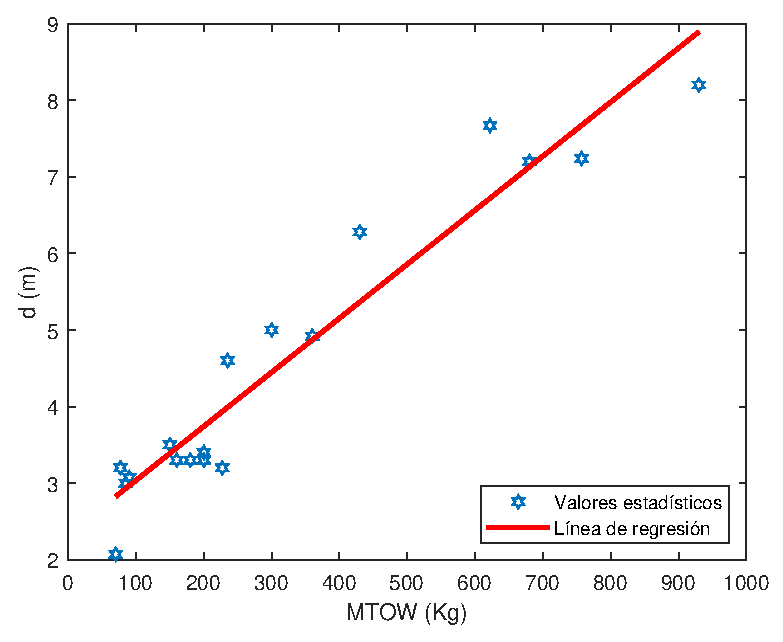
\includegraphics[width=90mm]{graficos/anald}
	\caption{Relación entre los diámetros de las palas de los helicópteros y sus MTOW junto a su línea de tendencia.}
	\label{diamAS}
\end{figure}
\begin{figure}
	\centering
	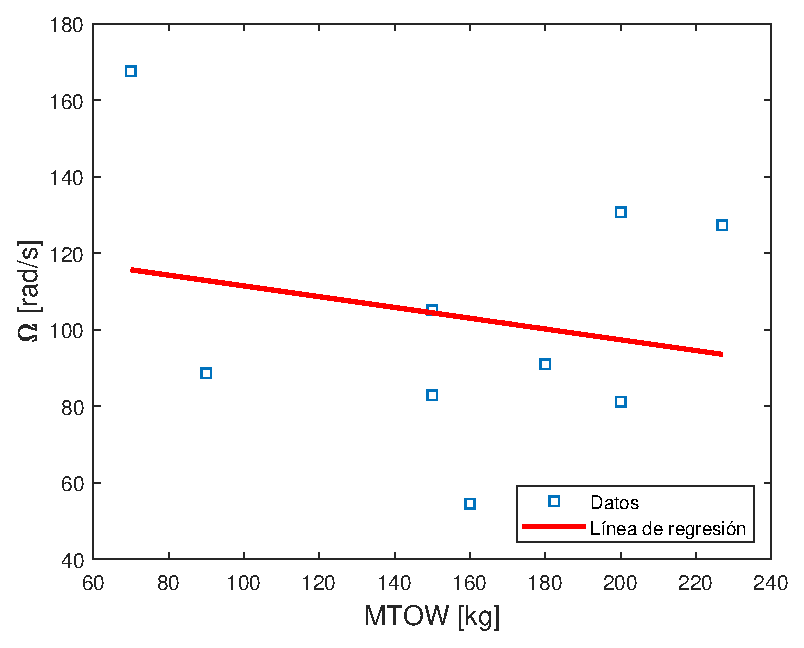
\includegraphics[width=90mm]{graficos/analomega}
	\caption{Relación entre las velocidades de giro del rotor de los helicópteros y sus MTOW junto a su línea de tendencia.}
	\label{omegaAS}
\end{figure}
\begin{figure}
	\centering
	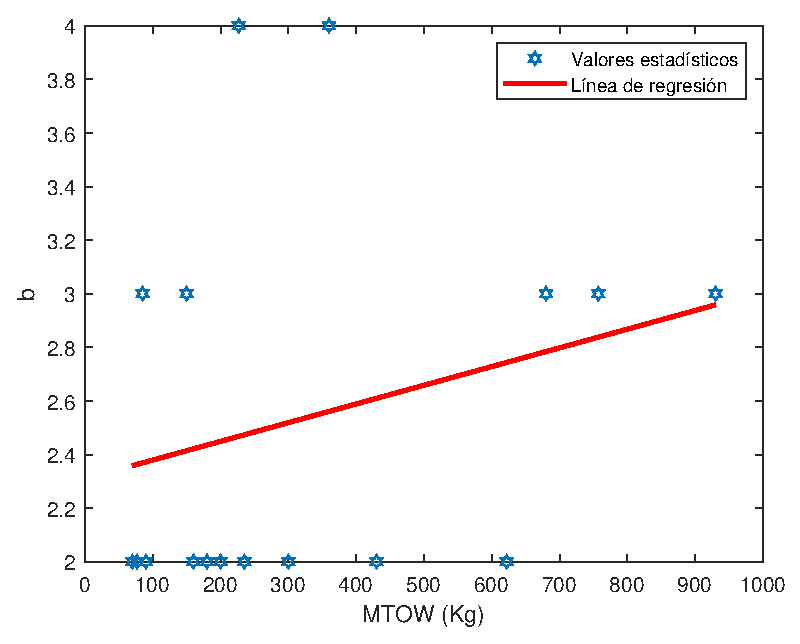
\includegraphics[width=90mm]{graficos/analb}
	\caption{Relación entre el número de palas del rotor principal de los helicópteros y sus MTOW junto a su línea de tendencia.}
	\label{bAS}
\end{figure}
\begin{figure}
	\centering
	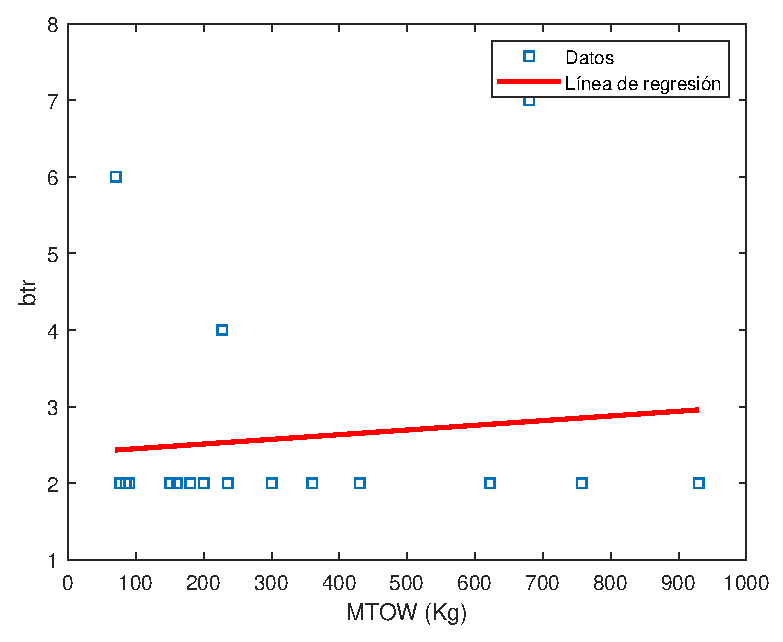
\includegraphics[width=90mm]{graficos/analbtr}
	\caption{Relación entre el número de palas del rotor antipar de los helicópteros y sus MTOW junto a su línea de tendencia.}
	\label{baAS}
\end{figure}
\begin{figure}
	\centering
	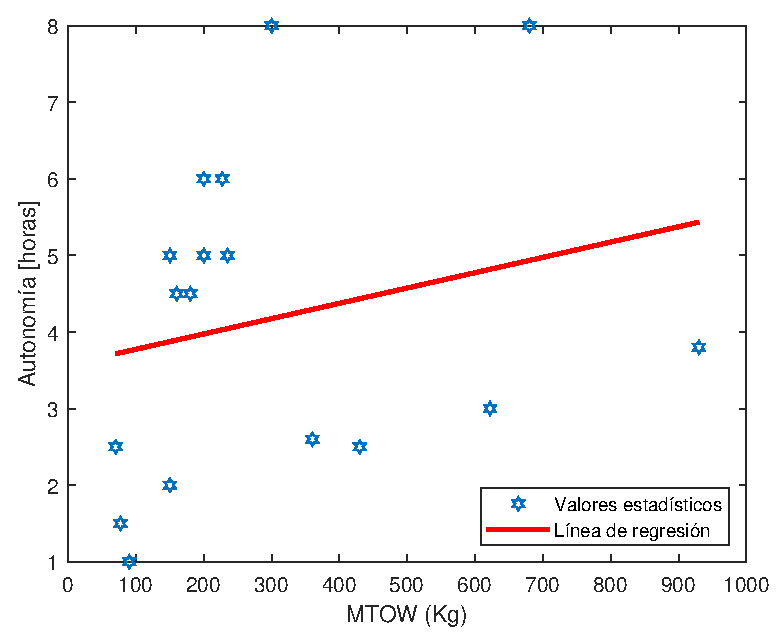
\includegraphics[width=90mm]{graficos/analaut}
	\caption{Relación entre las autonomías de los helicópteros y sus MTOW junto a su línea de tendencia.}
	\label{autAS}
\end{figure}
%\begin{figure}
%	\centering
%	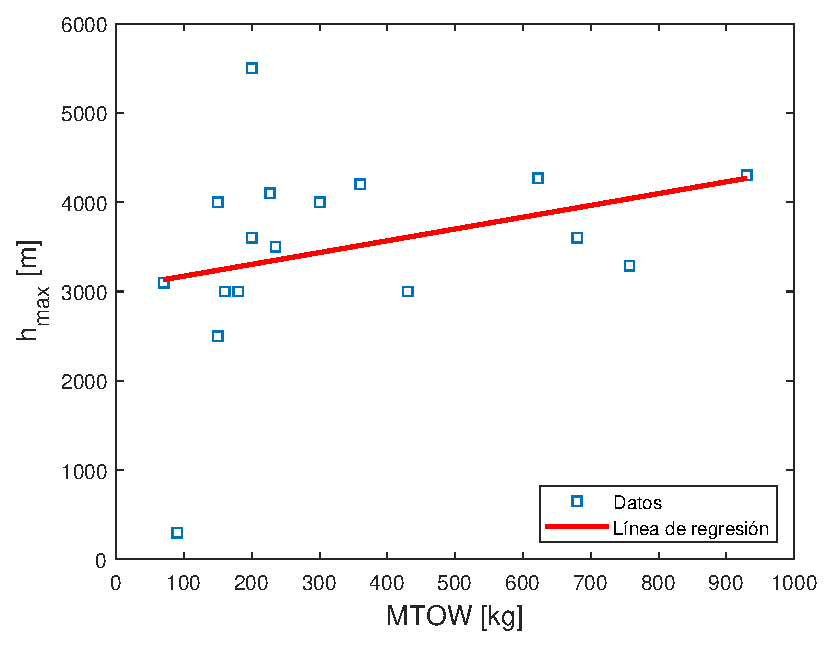
\includegraphics[width=90mm]{graficos/analtecho}
%	\caption{Relación entre los techos de vuelo de los helicópteros y sus MTOW junto a su línea de tendencia.}
%	\label{techoAS}
%\end{figure}
\begin{figure}
	\centering
	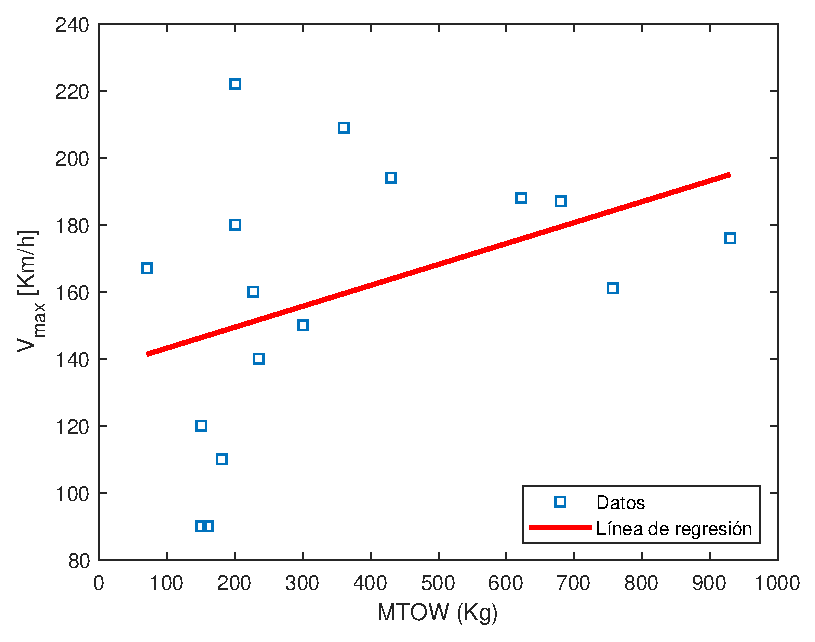
\includegraphics[width=90mm]{graficos/analv}
	\caption{Relación entre las velocidades máximas de avance de los helicópteros y sus MTOW junto a su línea de tendencia.}
	\label{vAS}
\end{figure}

Como se puede observar, muchos helicópteros comparten características aunque sus pesos sean muy distintos, y algunas líneas de tendencia se alejan considerablemente de los valores promedio para la zona que corresponde a 450 kg. Esto se debe, principalmente, a la falta de datos de referencia; los pocos desarrollos que se han dado de aeronaves de ala rotatoria en el entorno de pesos dado dificultan en gran medida la verificación de nuestro modelo al no existir una norma de diseño en la que basarnos. Los desarrollos han sido dispersos, así que los parámetros iniciales de diseño no se basarán únicamente en los valores de tendencia obtenidos estadísticamente, sino que más adelante se definirán los más problemáticos siguiendo otros criterios.
Algunos valores de referencia serán los siguientes:

\begin{itemize}
	\item $d$: 5,5 m
%	\item $\Omega$: 120 rad/s
	\item $b$: 2
	\item $b_{a}$: 2
	\item $t_{e}$: 4.5 horas
%	\item $h_{max}$: 3200 m
	\item $V_{max}$: 190 m/s
\end{itemize}

Queda patente que en algunos casos, se han aproximado los valores omitiendo las líneas de tendencia, usando en su lugar los valores de los helicópteros cuyos MTOW son más próximos al de la aeronave a diseñar.
La autonomía y velocidad máxima no son parámetros de diseño, sino que podrán usarse como referencia para comparar con los valores de la aeronave a diseñar para comprobar si se aproxima a los diseños actuales o no.
La velocidad de giro del rotor principal si sería un parámetro de diseño, pero debido a la falta de datos para hacer un cálculo estadístico, más adelante planteará un método para calcularla.
